\chapter{Fundamentação Teórica}
\label{cap:fundamentacao}

Este capítulo apresenta os conceitos de \english{\acrfull{csr}} e \english{\acrfull{ssr}}, abordando os princípios fundamentais do desenvolvimento web relacionados à renderização de conteúdo. Também são discutidos aspectos como \acrshort{seo}, desempenho, infraestrutura de serviços e impacto na experiência do usuário, estabelecendo a base teórica para o estudo de caso desenvolvido neste trabalho.

\section{Fundamentos de Desenvolvimento Web}
\label{sec:fundamentos-devweb}
Para entender como as abordagens \acrshort{ssr} e \acrshort{csr} se inserem no cenário de desenvolvimento web, é fundamental revisar protocolos, modelos de arquitetura e ferramentas.
Os fundamentos de desenvolvimento web englobam os princípios, tecnologias e práticas essenciais para a criação e manutenção de aplicações acessíveis via internet. 

O desenvolvimento web baseia-se na arquitetura cliente-servidor, onde o cliente (geralmente um navegador) solicita recursos ao servidor, que processa essas requisições e retorna os dados necessários. Essa interação é mediada por protocolos como o 
\english{\acrfull{http}} , que define as regras de comunicação entre cliente e servidor.

As tecnologias fundamentais incluem \english{\acrfull{html}} para estruturação do conteúdo, \english{\acrfull{css}} para estilização e JavaScript para interatividade. Essas linguagens permitem a construção de interfaces dinâmicas e responsivas. Além disso, o desenvolvimento web envolve práticas como controle de versão, testes automatizados e integração contínua, que garantem a qualidade e a escalabilidade das aplicações \cite{fundamentosDevWeb}. 

\subsection{Arquitetura Cliente-Servidor}
\label{subsec:Arquitetura Cliente-Servidor}

A arquitetura cliente-servidor é um modelo amplamente adotado no desenvolvimento de aplicações web, caracterizado pela separação entre dois componentes principais: o \textbf{cliente}, responsável pela interface com o usuário, e o \textbf{servidor}, que processa solicitações e fornece os recursos necessários \cite{clienteServidorControlNet}.

Nesse modelo, os clientes — como navegadores em diferentes dispositivos — enviam requisições através da internet, enquanto os servidores respondem disponibilizando dados, arquivos e serviços. Essa divisão de responsabilidades favorece a escalabilidade, facilita a manutenção e permite que cliente e servidor operem em plataformas distintas~\cite{fundamentosDevWeb}.

A Figura~\ref{fig:cliente-servidor} ilustra, de forma simplificada, esse fluxo de comunicação entre cliente e servidor.

\begin{figure}[H]
  \centering
  \caption{Comunicação entre cliente e servidor.}
  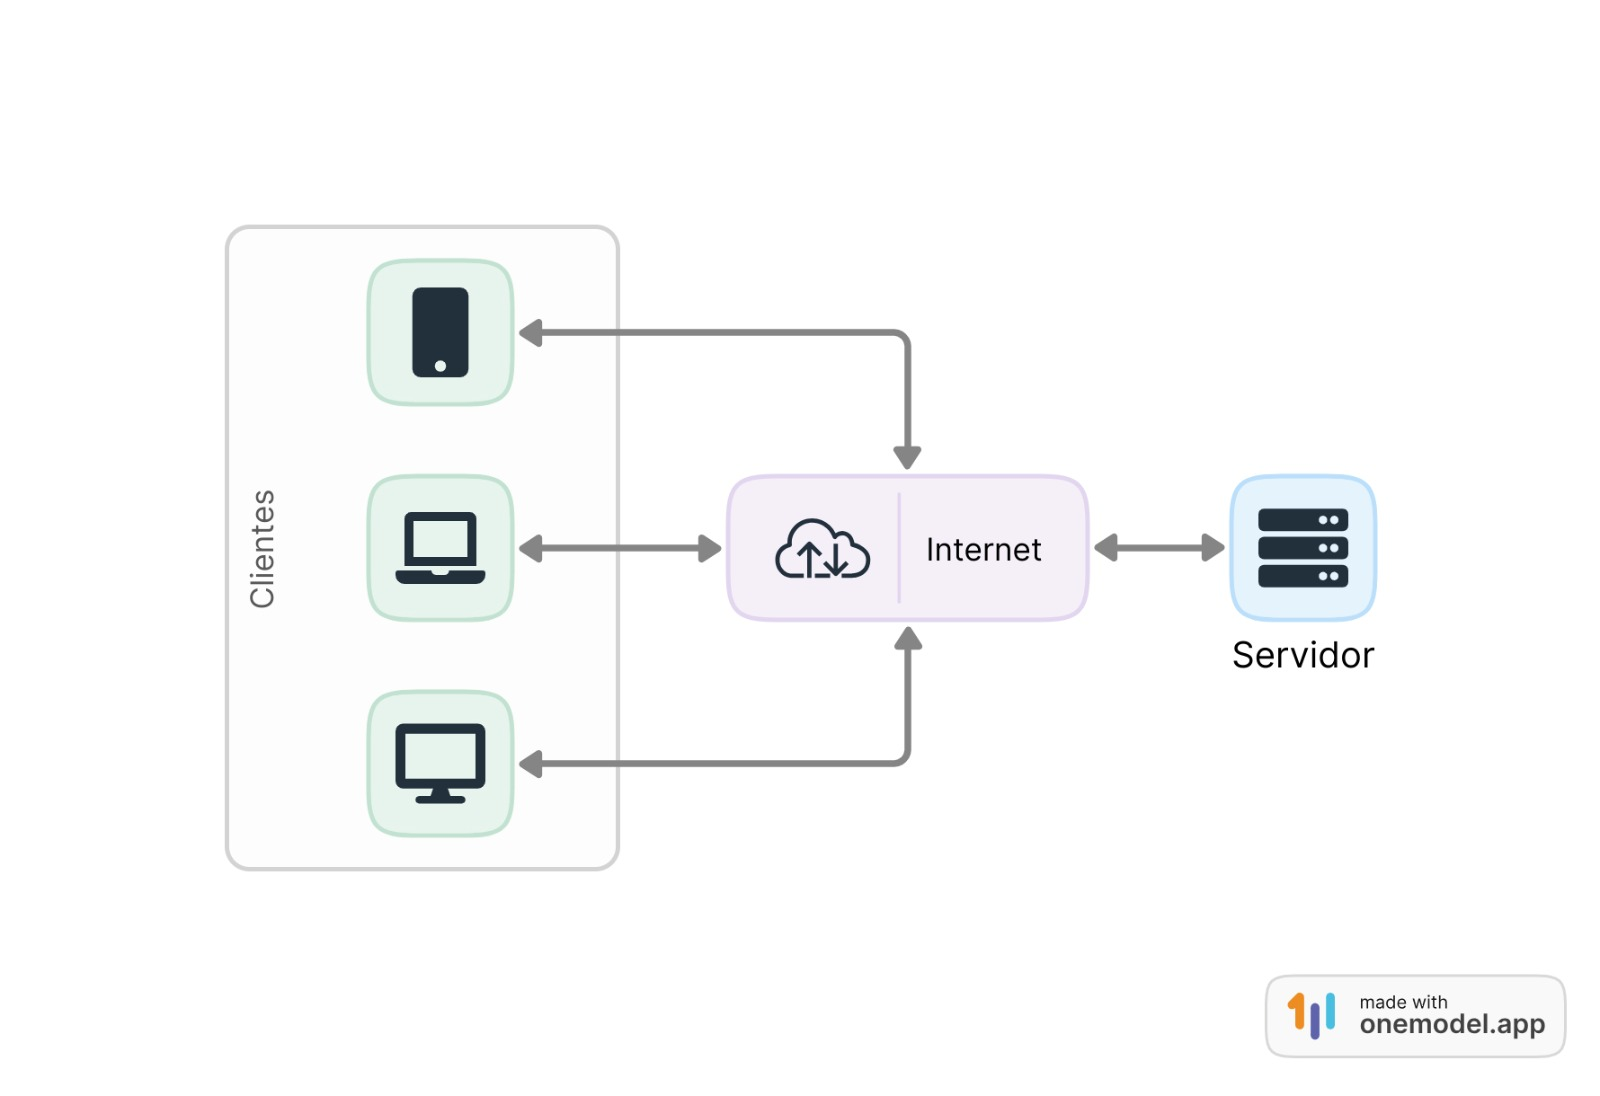
\includegraphics[width=0.8\textwidth]{media/cliente_servidor.jpeg}
  \legend{Fonte: \cite{fundamentosDevWeb} }
  \label{fig:cliente-servidor}
\end{figure}


A arquitetura cliente-servidor apresenta características que contribuem para sua ampla adoção em aplicações web. Entre elas, destaca-se a \textbf{distribuição de responsabilidades}, onde o servidor gerencia dados e processos mais complexos, enquanto o cliente lida com a interface e a interação com o usuário. 

Outro ponto relevante é a \textbf{independência entre plataformas}, possibilitada pelo uso de protocolos padronizados, o que permite a comunicação entre diferentes dispositivos e sistemas operacionais. Além disso, esse modelo favorece a \textbf{facilidade de manutenção}, já que atualizações podem ser feitas no servidor sem necessidade de intervenção nos dispositivos dos usuários.

Na web, essa arquitetura é implementada por padrão: navegadores atuam como clientes, enviando requisições \acrshort{http} que são processadas por servidores, os quais respondem com páginas e recursos solicitados~\cite{fundamentosDevWeb}.


\subsection{Protocolo \acrshort{http}}
\label{subsec:http}
O \textbf{Protocolo de Transferência de Hipertexto} (\acrshort{http}) é a base da comunicação na World Wide Web, definindo como clientes (navegadores) e servidores trocam informações. Ele especifica a estrutura das requisições e respostas, permitindo a recuperação de recursos como documentos \acrshort(html), imagens e vídeos \cite{mdn_http}.


 O \textbf{Funcionamento do \acrshort{http}}opera no modelo cliente-servidor, onde o cliente inicia uma requisição e o servidor responde com os recursos solicitados ou mensagens de erro, se aplicável. Cada interação consiste em uma mensagem de requisição do cliente e uma mensagem de resposta do servidor. As mensagens \acrshort{http} são compostas por:

\begin{itemize}
    \item \textbf{Linha de início:} Indica o método \acrshort{http} (como \texttt{GET} ou \texttt{POST}) e o caminho do recurso.
    \item \textbf{Cabeçalhos:} Fornecem informações adicionais sobre a requisição ou resposta, como tipo de conteúdo e codificação.
    \item \textbf{Corpo:} Contém os dados enviados ou recebidos, sendo opcional dependendo do método utilizado.
\end{itemize}

\begin{flushright}
    \cite{mdn_http}
\end{flushright}


\textbf{Métodos \acrshort{http}} são operações definidas pelo protocolo que especificam a ação a ser realizada em um recurso. Os métodos mais comuns incluem:

\begin{itemize}
    \item \textbf{GET:} Solicita a representação de um recurso específico. Requisições GET devem ser utilizadas apenas para recuperar dados.
    \item \textbf{POST:} Envia dados ao servidor para processamento, como o envio de formulários.
    \item \textbf{PUT:} Atualiza um recurso existente ou cria um novo se não existir.
    \item \textbf{DELETE:} Remove um recurso específico.
    \item \textbf{HEAD:} Similar ao GET, mas solicita apenas os cabeçalhos da resposta, sem o corpo.
\end{itemize}
Cada método possui uma finalidade específica e deve ser utilizado conforme a necessidade da aplicação \cite{wikipedia_http}.


\textbf{Códigos de Status \acrshort{http}} são códigos de três dígitos que indicam o resultado de uma requisição feita pelo cliente ao servidor. Eles são agrupados em cinco classes principais:

\begin{itemize}
    \item \textbf{1xx (Informativo):} Indica que a requisição foi recebida e o processo continua.
    \item \textbf{2xx (Sucesso):} Indica que a requisição foi bem-sucedida. Exemplo: 200 OK.
    \item \textbf{3xx (Redirecionamento):} Indica que é necessário tomar medidas adicionais para completar a requisição. Exemplo: 301 Moved Permanently.
    \item \textbf{4xx (Erro do Cliente):} Indica que houve um erro na requisição do cliente. Exemplo: 404 Not Found.
    \item \textbf{5xx (Erro do Servidor):} Indica que o servidor falhou ao processar uma requisição válida. Exemplo: 500 Internal Server Error.
\end{itemize}

Esses códigos auxiliam na identificação e resolução de problemas durante a comunicação \acrshort{http} \cite{mdn_http}.


\textbf{Evolução do \acrshort{http}} refere-se às revisões progressivas do protocolo com o objetivo de aprimorar sua eficiência, segurança e desempenho ao longo do tempo. As principais versões são:

\begin{itemize}
    \item \textbf{HTTP/1.0:} Primeira versão oficial do protocolo, em que cada requisição exigia uma nova conexão com o servidor.
    \item \textbf{HTTP/1.1:} Introduziu conexões persistentes, permitindo múltiplas requisições por conexão. Trouxe também melhorias no controle de cache e suporte a novos métodos.
    \item \textbf{HTTP/2:} Implementou multiplexação, compressão de cabeçalhos e priorização de fluxos, resultando em uma transferência de dados mais rápida e eficiente.
    \item \textbf{HTTP/3:} Baseado no protocolo \acrshort{quic}, substitui o \acrshort{tcp} pelo \acrshort{udp}, oferecendo conexões mais rápidas e seguras, com menor latência e melhor desempenho em redes instáveis.
\end{itemize}

Essas atualizações refletem a evolução das necessidades da web e a busca por protocolos mais robustos e otimizados \cite{cloudflare_http}.

\textbf{\acrshort{http} e \acrshort{https}} representam protocolos utilizados para comunicação na web, com a principal distinção centrada na segurança da transmissão dos dados.

O \textbf{\english{\acrfull{https}}} é uma extensão do \acrshort{http} que adiciona uma camada de proteção por meio do protocolo \english{\acrfull{tls}} ou, anteriormente, \english{\acrfull{ssl}}. Essa camada de segurança garante a confidencialidade, integridade e autenticidade dos dados trafegados entre cliente e servidor. 

A criptografia utilizada impede que terceiros acessem ou modifiquem as informações transmitidas, o que é fundamental em transações sensíveis, como cadastros, pagamentos e autenticações. Além disso, o uso de \textit{certificados digitais} garante que o site visitado é realmente aquele que afirma ser, protegendo os usuários contra ataques como o \textit{man-in-the-middle}\footnote{Um ataque \textit{man-in-the-middle} ocorre quando um invasor intercepta e possivelmente altera a comunicação entre duas partes que acreditam estar se comunicando diretamente. Isso pode permitir que o invasor capture informações sensíveis ou injete dados maliciosos na comunicação.\cite{wikipedia_man_in_the_middle}}.

Enquanto o \acrshort{http} tradicional opera normalmente na porta \acrshort{tcp} 80, o \acrshort{https} utiliza, por convenção, a porta 443. Atualmente, o uso do \acrshort{https} é fortemente recomendado — e até exigido por navegadores modernos — como padrão de segurança para qualquer aplicação web, contribuindo para a privacidade e confiança dos usuários \cite{wikipedia_http}.

\subsection{\acrshort{html}, \acrshort{css} e JavaScript}
\label{subsec:html-css-js}


O desenvolvimento frontend, conforme definido por \citeonline{aws_frontend_backend}, refere-se à camada de apresentação de uma aplicação web — a interface gráfica com a qual os usuários interagem diretamente, composta por menus, botões, formulários e outros elementos visuais. Essa camada baseia-se em um conjunto de tecnologias fundamentais que operam em conjunto para fornecer estrutura, estilo e interatividade às páginas: \acrshort{html}, \acrshort{css} e JavaScript. Cada uma dessas linguagens desempenha um papel específico e complementar, sendo essenciais tanto em abordagens tradicionais quanto em técnicas modernas como o \acrshort{csr}.


\textbf{\acrfull{html}} é a linguagem de marcação padrão para a criação da estrutura de páginas web. Através de um conjunto de elementos (ou \textit{tags}), o \acrshort{html} organiza e define o conteúdo exibido ao usuário, como textos, imagens, links, formulários e tabelas. Além de estruturar visualmente o documento, o \acrshort{html} também confere semântica aos elementos, facilitando a indexação por motores de busca e promovendo acessibilidade para leitores de tela. Elementos como \texttt{<header>}, \texttt{<main>}, \texttt{<article>} e \texttt{<footer>} exemplificam essa função semântica~\cite{alura_htmlcssjs}.

\textbf{\acrfull{css}} é a linguagem responsável pela estilização das páginas web. Com o \acrshort{css}, define-se a aparência dos elementos estruturados no \acrshort{html}, controlando propriedades visuais como cores, fontes, espaçamentos, tamanhos e posicionamentos. O \acrshort{css} permite ainda a construção de layouts complexos e responsivos, adaptando o conteúdo para diferentes tamanhos de tela e dispositivos. A separação entre estrutura (\acrshort{html}) e estilo (\acrshort{css}) é um dos pilares das boas práticas em desenvolvimento web, promovendo manutenibilidade, reutilização e modularidade do código.

Entre os recursos modernos do \acrshort{css}, destacam-se os seletores avançados, variáveis \acrshort{css}, pseudo-classes, animações e as funcionalidades de \textit{Flexbox} e \textit{Grid}, que facilitam a criação de interfaces ricas e adaptáveis~\cite{herocode_diferencas}.

\textbf{JavaScript} é uma linguagem de programação interpretada, orientada a objetos e baseada em eventos, amplamente utilizada para adicionar interatividade e dinamismo às páginas web. Por meio da manipulação da \textit{\acrfull{dom}}, permite implementar funcionalidades como respostas a cliques, envio de formulários, movimentações do mouse, digitação, animações, validações e atualizações em tempo real, enriquecendo significativamente a experiência do usuário~\cite{alura_htmlcssjs}. Além disso, possibilita o carregamento assíncrono de dados com a técnica \textit{AJAX} (\textit{Asynchronous JavaScript and XML}), evitando recarregamentos completos da página.

JavaScript é uma das três principais tecnologias da World Wide Web, juntamente com \acrshort{html} e \acrshort{css}, sendo essencial tanto em abordagens tradicionais quanto modernas. Nas aplicações baseadas em \acrshort{csr}, essa linguagem tem papel central, pois a renderização das páginas ocorre diretamente no navegador do usuário. Com a evolução do ecossistema JavaScript, surgiram bibliotecas e frameworks robustos como a biblioteca React e os frameworks Vue.js e Angular que facilitam o desenvolvimento de aplicações complexas com componentes reutilizáveis e gerenciamento eficiente de estado.

Adicionalmente, o JavaScript também pode ser executado no lado do servidor (\acrshort{ssr}) por meio de ambientes como o Node.js — uma plataforma de código aberto e multiplataforma baseada em eventos e não bloqueante, ideal para aplicações escaláveis e em tempo real~\cite{nodejs2025, js2025}. Isso permite o desenvolvimento de aplicações completas utilizando uma única linguagem em ambas as camadas, cliente e servidor.

A interação entre essas três tecnologias pode ser compreendida por meio de uma analogia: o \acrshort{html} representa a estrutura de um corpo (esqueleto), o \acrshort{css} corresponde à sua aparência externa (pele, roupas, estilo), enquanto o JavaScript age como os músculos e o sistema nervoso, controlando os movimentos e respostas interativas da aplicação. A Figura~\ref{fig:html-css-js} ilustra essa relação.

\begin{figure}[H]
  \centering
  \caption{Analogia entre HTML, CSS e JavaScript e os componentes de um corpo humano.}
  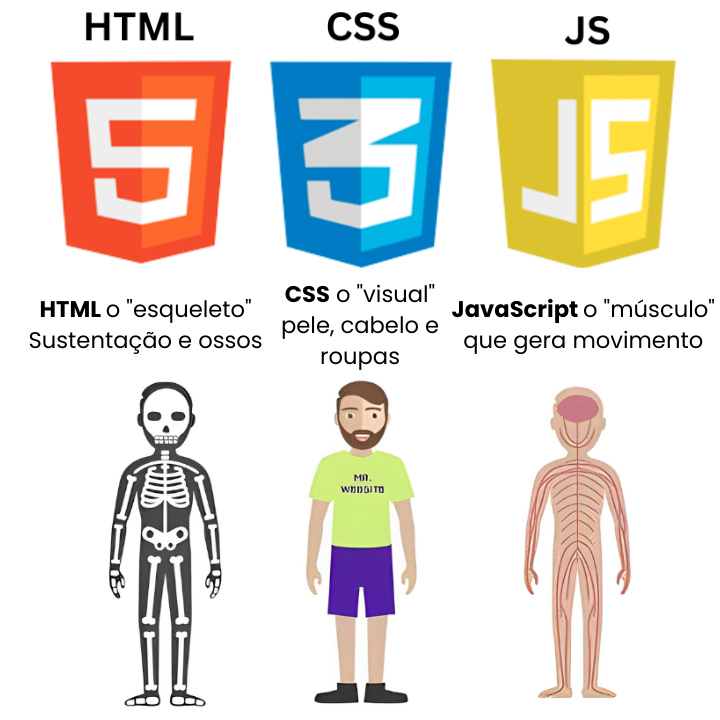
\includegraphics[width=0.6\textwidth]{media/html_css_js_analogia.png}
  \legend{Fonte: \cite{herocode_diferencas}.}
  \label{fig:html-css-js}
\end{figure}

Portanto, o domínio dessas três tecnologias é indispensável para qualquer desenvolvedor web. Elas formam o alicerce sobre o qual se constroem interfaces acessíveis, performáticas e envolventes, sendo empregadas tanto em aplicações renderizadas no servidor (\acrshort{ssr}) quanto no cliente (\acrshort{csr}), com adaptações específicas conforme a abordagem escolhida.


\section{\english{Client-Side Rendering} (\acrshort{csr})}
\label{subsec:csr}

A \textbf{\english{\acrfull{csr}}} é uma técnica em que a geração da interface e do conteúdo final ocorre diretamente no navegador do usuário, utilizando JavaScript. Nessa abordagem, o servidor envia um arquivo \english{\acrfull{html}} mínimo, contendo apenas a estrutura básica da página e referências a arquivos de estilo e scripts.{\cite{atori2024}}

Segundo \citeonline{atori2024}, o processo de renderização no cliente segue as seguintes etapas:

\begin{enumerate}
    \item O servidor envia uma página \acrshort{html} em branco contendo apenas links para os arquivos \english{\acrfull{css}} e JavaScript.
    \item O navegador interpreta o \acrshort{html} e constrói a árvore do \english{\acrfull{dom}}
    \item Os arquivos de estilo (\acrshort{css}) e script (JavaScript) são baixados pelo navegador.
    \item A aplicação é renderizada dinamicamente pelo JavaScript, incluindo elementos visuais como texto, imagens e botões.
    \item O conteúdo da página é atualizado de forma interativa conforme o usuário interage com a aplicação.
\end{enumerate}

Esse modelo é comumente utilizado em aplicações \english{\acrfull{spa}}, nas quais o carregamento inicial é seguido por atualizações dinâmicas sem recarregamento da página. Ferramentas como a biblioteca React, e frameworks como Vue.js, Angular e Svelte são amplamente utilizadas para implementar \acrshort{csr}, permitindo o desenvolvimento de interfaces dinâmicas, interativas e responsivas.


A renderização no lado do cliente (\acrshort{csr}) é especialmente vantajosa em aplicações que exigem alta interatividade e atualizações frequentes de conteúdo, como redes sociais, plataformas de streaming e jogos online. No entanto, essa abordagem pode apresentar desvantagens em termos de desempenho inicial e \acrshort{seo}, uma vez que o conteúdo só é exibido após a execução do JavaScript, o que pode impactar negativamente a indexação por motores de busca e a experiência do usuário em conexões lentas \cite{atori2024}.

\begin{figure}[h!]
    \centering
    \caption{Etapas do método de renderização no lado do cliente}
    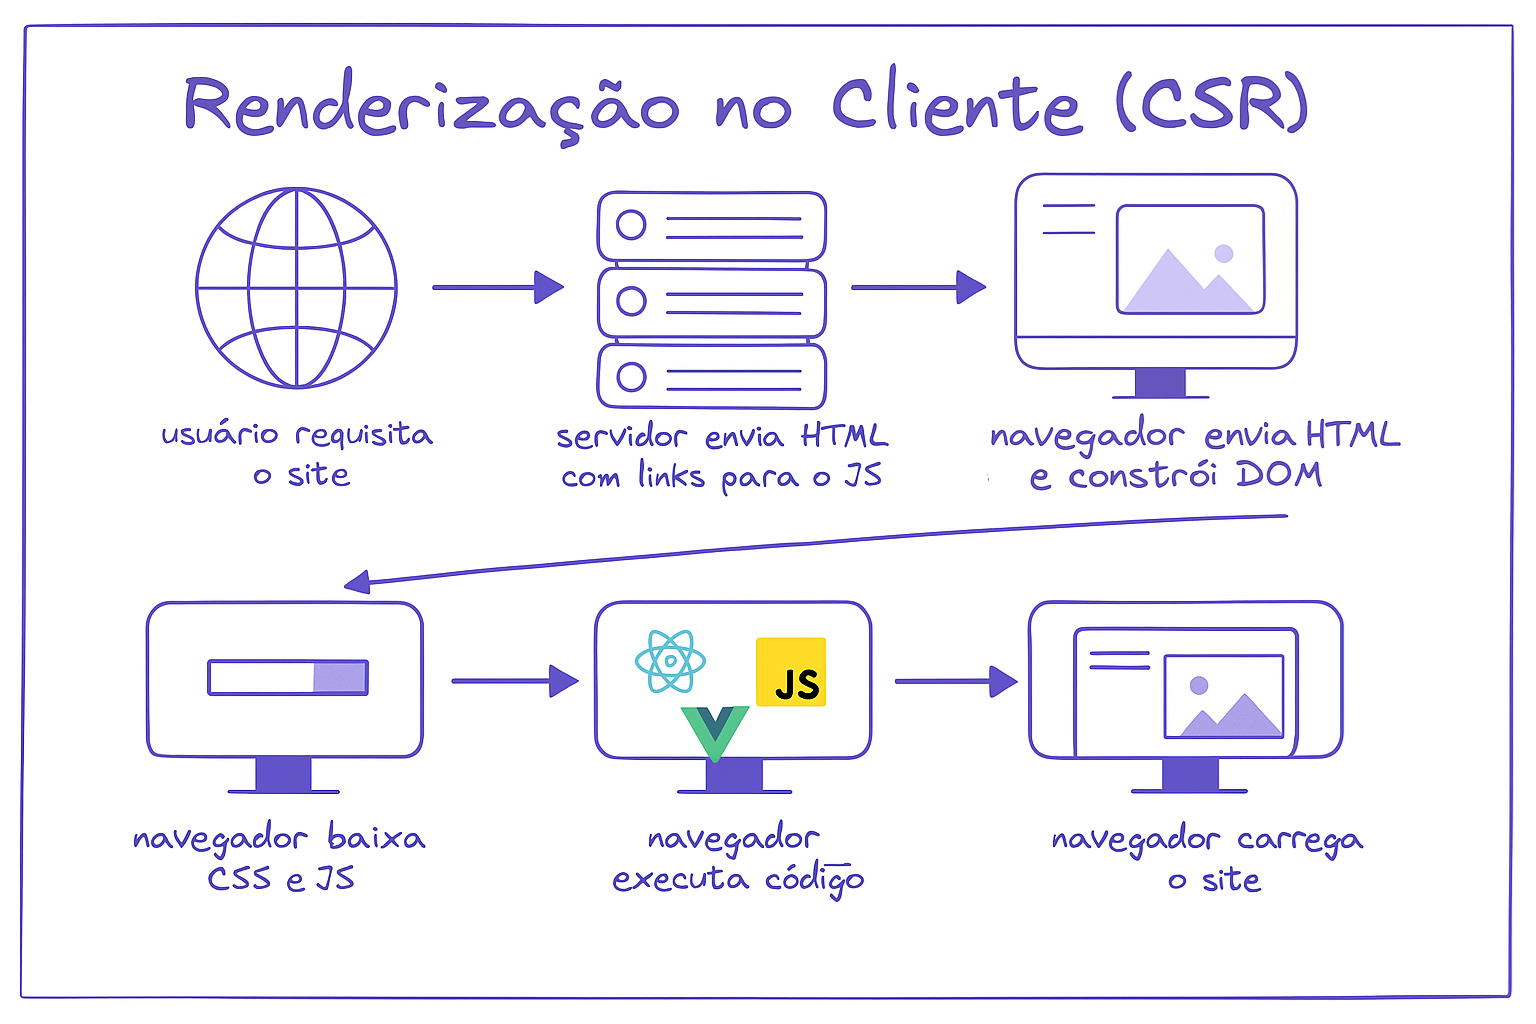
\includegraphics[width=0.8\textwidth]{media/client_side_rendering.png}
    \legend{Fonte: \cite{atori2024} (adaptado)}
    \label{fig:client_side_rendering}
\end{figure}


A \autoref{fig:client_side_rendering} ilustra visualmente o fluxo completo da renderização no lado do cliente (\acrshort{csr}). O processo é iniciado quando o usuário acessa o site em questão. Em resposta, o servidor envia o arquivo \acrshort{html} básico, contendo apenas links para os arquivos de estilo \acrshort{css} e scripts JavaScript responsáveis por carregar e renderizar o conteúdo da aplicação.

Na sequência, o navegador interpreta esse \acrshort{html} e constrói a estrutura da página por meio da árvore \acrshort{dom}. No entanto, o conteúdo principal ainda não está visível. O navegador então precisa baixar os arquivos de estilo (\acrshort{css}) e os scripts JavaScript referenciados no documento inicial.

Com os scripts carregados, o navegador executa o código JavaScript, que normalmente utiliza bibliotecas ou frameworks como React ou Vue para gerar dinamicamente o conteúdo da aplicação. Somente após essa etapa o conteúdo completo do site é finalmente exibido ao usuário, quando o navegador conclui o processo de renderização e o site é carregado completamente.

\begin{codigo}[H]
  \begin{lstlisting}[language=html]
<!DOCTYPE html>
<html lang="en">
<head>
  <meta charset="utf-8">
  <title>CryptoWebsite</title>
  <base href="/">
  <meta name="viewport" content="width=device-width, initial-scale=1">
  <link rel="icon" type="image/x-icon" href="favicon.ico">
  <style>*,*:before,*:after{margin:0;padding:0;box-sizing:border-box;
    font-family:Inter,sans-serif}html{font-size:62.5%}</style>
  <link rel="stylesheet" href="styles.9d4c7581c7242.css">
</head>
<body>
  <app-root></app-root>
  <script src="runtime.6170988ad52a05db.js" type="module"></script>
  <script src="polyfills.574970d5ec4bdb97.js" type="module"></script>
  <script src="main.202d37bb6740400e.js" type="module"></script>
</body>
</html>
\end{lstlisting}
  \caption{Exemplo de HTML mínimo em aplicação Angular com CSR}
  \label{lst:angular_html}
\end{codigo}

Esse padrão é típico de aplicações \acrshort{spa}, onde todo o conteúdo é inserido dinamicamente a partir da execução dos arquivos JavaScript. O elemento \texttt{<app-root>} funciona como ponto de entrada da aplicação, sendo substituído no navegador pelos componentes definidos no framework Angular. {\cite{atori2024}}


\section{\english{Server-Side Rendering} (\acrshort{ssr})}
\label{subsec:ssr}

A \textbf{\english{\acrfull{ssr}}} é uma abordagem em que a geração do conteúdo e da interface ocorre integralmente no servidor antes de ser enviada ao navegador do cliente. Ou seja, o servidor processa a lógica da aplicação, obtém dados necessários (por exemplo, em bancos de dados ou \emph{APIs}) e retorna ao cliente um arquivo \english{\acrshort{html}} já renderizado. Dessa forma, o navegador exibe imediatamente a página completa, sem precisar executar \emph{scripts} para montar o conteúdo inicial \cite{atori2024}. 

Segundo \citeonline{atori2024}, o processo típico de renderização no lado do servidor pode ser descrito em quatro etapas principais:

\begin{enumerate}
    \item O servidor recebe uma requisição para uma página e recupera os dados necessários para compor seu conteúdo (por exemplo, produtos de uma base de dados ou artigos de um blog).
    \item O servidor insere esses dados em um \emph{template} \acrshort{html}, gerando a estrutura final da página.
    \item Em seguida, o servidor aplica estilos e finaliza a renderização, resultando em um documento \acrshort{html} completamente montado.
    \item Por fim, esse documento \acrshort{html} é enviado ao navegador do usuário, exibindo a página prontamente, sem a necessidade de executar \emph{JavaScript} durante o carregamento inicial.
\end{enumerate}

Nesse modelo, a fase de hydration\footnote{Hydration é uma etapa essencial no \acrshort{ssr}, em que o JavaScript torna interativo o conteúdo HTML previamente renderizado no servidor.} ocorre após o carregamento inicial da página. costuma ocorrer após a entrega do conteúdo estático. Significa que, assim que o arquivo \acrshort{html} é carregado e mostrado ao usuário, o \emph{JavaScript} do lado do cliente assume o controle para tratar as interações e atualizações dinâmicas subsequentes. Dessa forma, o \acrshort{ssr} beneficia tanto o primeiro acesso (tornando o conteúdo visível rapidamente) quanto o \acrshort{seo}, por exibir ao rastreador dos mecanismos de busca um código \acrshort{html} completo. \cite{atori2024}.

\begin{figure}[H]
  \centering
  \caption{Etapas do método de renderização no lado do servidor}
  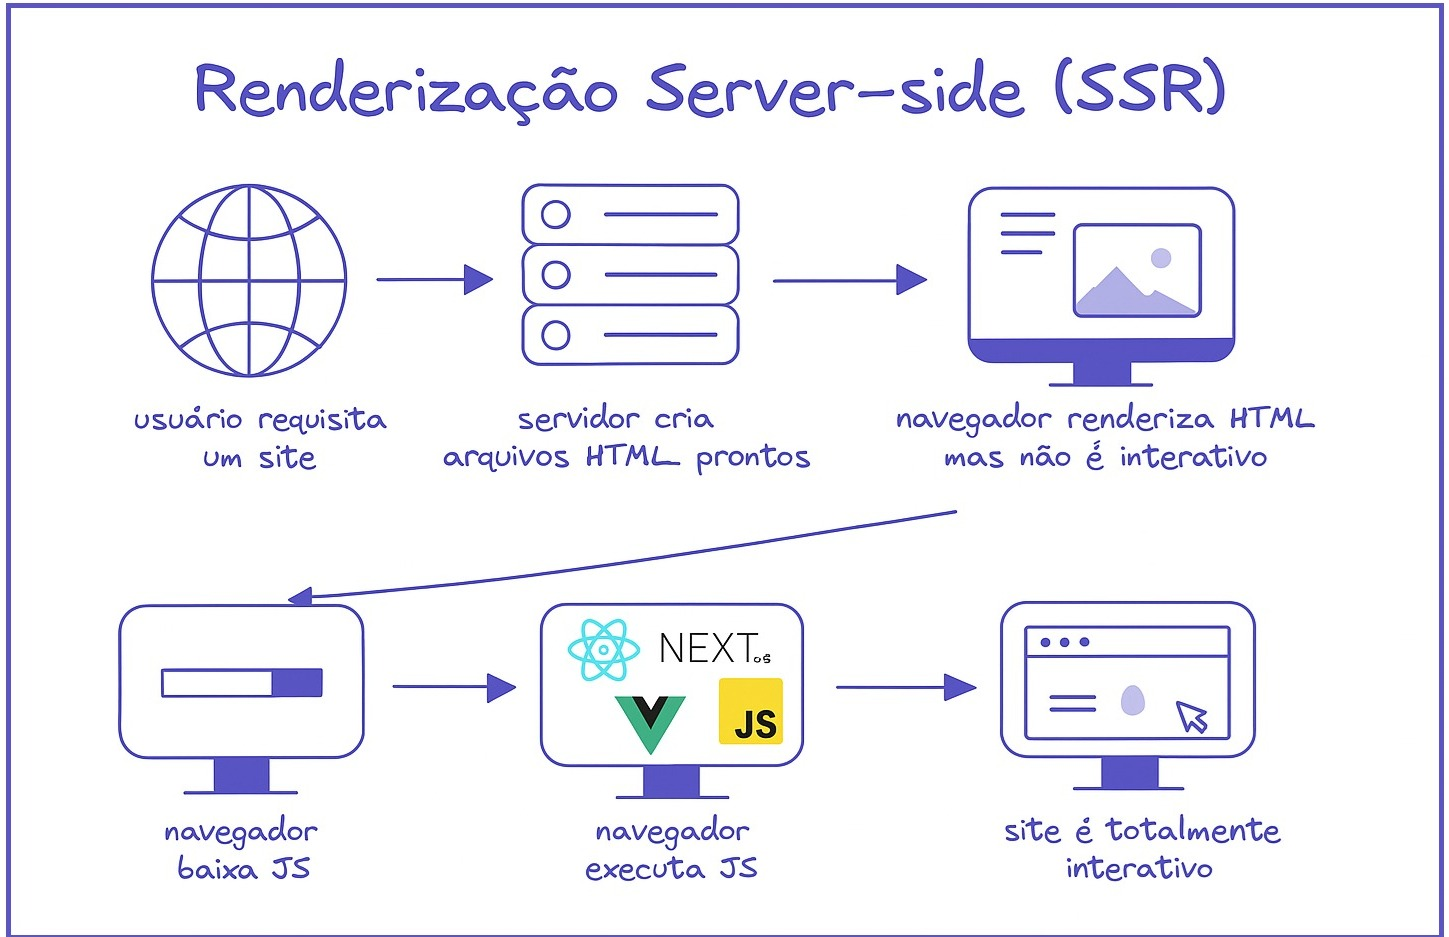
\includegraphics[width=0.8\textwidth]{media/server_side_rendering.jpeg}
  \legend{Fonte: \cite{atori2024} (adaptado)}
  \label{fig:server_side_rendering}
\end{figure}

A \autoref{fig:server_side_rendering} ilustra o fluxo de uma aplicação \acrshort{ssr}. Ao receber a requisição, o servidor gera a página completa em \acrshort{html} e a envia ao cliente. Essa estratégia costuma ser vantajosa em cenários onde o carregamento inicial rápido e a indexação por motores de busca são prioridades, como em sites de e-commerce e páginas de \emph{landing}, permitindo que o usuário visualize o conteúdo de forma imediata. 

\emph{Meta-frameworks} como Next.js, Nuxt.js, SvelteKit, Angular Universal, Remix, Astro e Qwik são amplamente utilizados para construir aplicações com suporte a \acrshort{ssr}. Esses frameworks operam em um nível superior aos tradicionais (como React, Vue ou Svelte), agregando funcionalidades comuns ao desenvolvimento web, como roteamento, pré-renderização, recuperação de dados e \emph{hydration} podendo oferecer uma estrutura mais completa, opinativa e voltada à escalabilidade.

O \acrshort{ssr} é especialmente útil em aplicações que exigem um carregamento inicial rápido e uma boa indexação por motores de busca, como sites de e-commerce, blogs e páginas de \emph{landing}. Essa abordagem permite que o usuário visualize o conteúdo imediatamente, sem esperar pela execução do JavaScript. Além disso, o \acrshort{ssr} melhora a \acrshort{seo}, pois os mecanismos de busca conseguem indexar o conteúdo completo da página desde o início.

No \autoref{lst:nextjs_html}, pode-se observar que o arquivo \acrshort{html} já contém todo o \emph{markup} necessário para exibir o conteúdo da página. Assim que o navegador recebe esse arquivo, o usuário já visualiza o cabeçalho, o texto e o layout definidos. Posteriormente, o \emph{JavaScript} baixado (por exemplo, \texttt{main.js}) pode entrar em ação para lidar com eventos, rotas adicionais e atualizações dinâmicas, caso o desenvolvedor deseje funcionalidades mais interativas.

Por fim, aplicações \acrshort{ssr} tendem a apresentar melhor performance em termos de \emph{time-to-first-byte}\footnote{O \emph{time-to-first-byte} (TTFB) é uma métrica que mede o tempo decorrido entre o envio de uma solicitação HTTP pelo cliente e o recebimento do primeiro byte da resposta do servidor. Um TTFB menor indica maior rapidez na resposta do servidor, impactando diretamente na velocidade de carregamento da página e na experiência do usuário. \cite{ttfb-craig}} e de \emph{indexabilidade}\footnote{A \emph{indexabilidade} refere-se à capacidade dos motores de busca de rastrear e indexar o conteúdo de uma página web. Aplicações SSR, ao fornecerem conteúdo totalmente renderizado no servidor, facilitam a indexação eficiente pelos motores de busca, melhorando a visibilidade nos resultados de pesquisa. \cite{ttfb-oskay}} por motores de busca, ao mesmo tempo em que podem demandar maior carga de processamento no servidor. A escolha por \acrshort{ssr} ou não, portanto, depende do perfil da aplicação e das prioridades do projeto, considerando fatores como volume de tráfego, necessidade de interatividade e requisitos de otimização de conteúdo.

\begin{codigo}[H]
  \begin{lstlisting}[language=html]
    <!DOCTYPE html>
    <html lang="en">
    <head>
      <meta charset="utf-8">
      <title>My SSR App</title>
      <meta name="viewport" content="width=device-width, initial-scale=1">
      <style>
        /* Exemplo simples de estilo inline */
        body {
          margin: 0;
          font-family: Arial, sans-serif;
          background: #f6f6f6;
        }
        h1 { color: #333; }
      </style>
    </head>
    <body>
<!-- Conteudo ja processado e inserido no servidor -->
      <div id="__next">
        <header>
          <h1>Ola, mundo!</h1>
        </header>
        <main>
          <p>Este conteudo foi renderizado no servidor usando Next.js.</p>
        </main>
      </div>
      <!-- Scripts do Next.js para interacao no cliente -->
      <script src="/_next/static/chunks/main.js" defer></script>
    </body>
    </html>
  \end{lstlisting}
  \caption{Exemplo de HTML mínimo em aplicação Next.js com SSR}
  \label{cod:nextjs_html}
\end{codigo}


\section{Frameworks Web}
\label{sec:frameworks-web}

O uso de bibliotecas e frameworks no desenvolvimento web moderno proporciona ganhos significativos de produtividade, desempenho e organização de código. Eles abstraem operações complexas e oferecem estruturas padronizadas para construção de aplicações escaláveis. A escolha da ferramenta está diretamente relacionada à abordagem de renderização adotada, seja no lado do cliente (\acrshort{csr}) ou do servidor (\acrshort{ssr}).

\subsection{Bibliotecas JavaScript}
\label{subsec:bibliotecas-js}

Bibliotecas JavaScript são conjuntos de funcionalidades reutilizáveis que fornecem recursos específicos, permitindo que o desenvolvedor tenha maior controle sobre o fluxo da aplicação. Elas diferem dos frameworks por não imporem uma estrutura rígida, sendo mais flexíveis em sua aplicação.

\textbf{React} é um exemplo amplamente utilizado de biblioteca voltada para a criação de interfaces de usuário baseadas em componentes reutilizáveis. Desenvolvida pelo Facebook, React se destaca por sua abordagem declarativa, desempenho otimizado com o uso de um \textit{virtual DOM}, e ampla adoção na construção de aplicações com \acrshort{csr}. Apesar de muitas vezes ser chamado de framework, React é tecnicamente uma biblioteca, já que seu foco é exclusivamente a camada de visualização, deixando a cargo do desenvolvedor a escolha de ferramentas para rotas, estados e lógica de aplicação~\cite{react2025}.

\subsection{Frameworks para CSR}
\label{subsec:frameworks-csr}

No modelo \acrshort{csr}, a renderização da interface é realizada diretamente no navegador do usuário, após o carregamento dos arquivos JavaScript. Frameworks como os listados a seguir são amplamente utilizados para implementar essa abordagem:

\begin{itemize}
    \item \textbf{Vue.js}: framework progressivo para construção de interfaces web interativas. Seu foco está na camada de visualização, com curva de aprendizado acessível e estrutura modular~\cite{vue2025}.
    
    \item \textbf{Angular}: framework completo mantido pelo Google, baseado em TypeScript, que oferece arquitetura robusta e recursos integrados como injeção de dependência e roteamento~\cite{angular2025}.
    
    \item \textbf{Svelte}: framework que realiza a compilação dos componentes no momento do build, eliminando a necessidade de um \textit{virtual DOM}, o que reduz o tempo de carregamento e o uso de recursos do navegador~\cite{svelte2025}.
\end{itemize}

Esses frameworks tornam o desenvolvimento com \acrshort{csr} mais eficiente e sustentável, proporcionando experiências ricas ao usuário com foco em interatividade e responsividade.

\subsection{Meta-frameworks para SSR}
\label{subsec:frameworks-ssr}

Para aplicações com foco em renderização no lado do servidor, os \emph{meta-frameworks} oferecem soluções completas, otimizando tanto o desempenho inicial quanto a indexabilidade em mecanismos de busca. Eles operam sobre frameworks tradicionais (como Vue ou Svelte) ou bibliotecas (como React), incorporando funcionalidades essenciais como roteamento, pré-renderização, recuperação de dados e \textit{hydration}.

\begin{itemize}
    \item \textbf{Next.js}: baseado em React, fornece recursos para \acrshort{ssr}, geração de sites estáticos e suporte a APIs integradas~\cite{nextjs2024}.
    
    \item \textbf{Nuxt.js}: extensão do Vue.js que oferece SSR, geração estática e arquitetura modular~\cite{nuxtjs2024}.
    
    \item \textbf{SvelteKit}: baseado em Svelte, permite renderização no servidor e no cliente, com foco em simplicidade e desempenho~\cite{sveltekit2024}.
    
    \item \textbf{Angular Universal}: solução oficial para SSR em Angular, melhora a indexação e o tempo de carregamento inicial~\cite{angularuniversal2024}.
    
    \item \textbf{Remix}: framework full-stack para React que adota um modelo de dados centrado em carregadores e ações~\cite{remix2024}.
    
    \item \textbf{Astro}: framework moderno que carrega apenas o JavaScript necessário, permitindo uso híbrido de componentes React, Vue, Svelte e outros~\cite{astro2024}.
    
    \item \textbf{Qwik}: introduz o conceito de aplicações \textit{resumíveis}, com SSR e carregamento progressivo de interatividade~\cite{qwik2024}.
\end{itemize}

Esses meta-frameworks são especialmente indicados para aplicações que priorizam SEO, acessibilidade e desempenho no primeiro carregamento, como páginas institucionais, lojas virtuais e blogs.

\subsection{Comparativo entre Frameworks CSR e SSR}
\label{subsec:comparativo-frameworks}

\begin{table}[H]
\centering
\caption{Comparação entre frameworks para CSR e SSR}
\label{tab:comparativo-frameworks}
\begin{tabular}{|p{3cm}|p{5.5cm}|p{5.5cm}|}
\hline
\textbf{Critério} & \textbf{Frameworks CSR (Vue, Angular, Svelte)} & \textbf{Meta-frameworks SSR (Next.js, Nuxt, SvelteKit, etc.)} \\
\hline
\textbf{Renderização Inicial} & O conteúdo é montado no navegador após o carregamento do JavaScript & O conteúdo é gerado no servidor e entregue já renderizado ao navegador \\
\hline
\textbf{Tempo de Carregamento} & Maior tempo de carregamento inicial (dependente do JS) & Melhor desempenho no carregamento inicial (TTFB menor) \\
\hline
\textbf{SEO} & Pode ser limitado, pois bots podem não processar JavaScript adequadamente & Excelente, já que o HTML completo está disponível para rastreadores \\
\hline
\textbf{Interatividade} & Alta, com foco em aplicações ricas e dinâmicas & Boa, com necessidade de \textit{hydration} após o carregamento \\
\hline
\textbf{Complexidade de Infraestrutura} & Menor, geralmente servido por CDNs e arquivos estáticos & Maior, exige servidores para processar cada requisição \\
\hline
\textbf{Casos de Uso Ideais} & SPAs, dashboards, aplicações com muitas interações em tempo real & Landing pages, blogs, e-commerces, sites que dependem de SEO \\
\hline
\end{tabular}
\end{table}


% \subsection{Modelos de Arquitetura Web}
% \label{subsec:modelos-arq-web}
% Os modelos arquiteturais variam conforme os requisitos de escalabilidade, manutenção e desempenho:

% \begin{itemize}
%     \item \textbf{Arquitetura Monolítica}: Um único projeto concentra \textit{frontend} e \textit{backend}, frequentemente usando \acrshort{ssr}. Possui inicialização simples, mas pode tornar-se complexo de manter e escalar.
%     \item \textbf{Microserviços}: Divide a aplicação em múltiplos serviços independentes. Cada serviço pode escolher a melhor abordagem de renderização (SSR ou CSR), facilitando a escalabilidade seletiva.
%     \item \textbf{Serverless}: As funções são executadas sob demanda em plataformas de nuvem, onde a renderização pode ocorrer tanto no servidor (funções que retornam HTML) quanto no cliente (ao entregar apenas APIs).
% \end{itemize}

% \subsection{Ferramentas e \textit{Frameworks}}
% \label{subsec:ferramentas-frameworks}
% O ecossistema de desenvolvimento web oferece diversas ferramentas que simplificam \acrshort{ssr} e \acrshort{csr}:

% \begin{itemize}
%     \item \textbf{\acrshort{ssr}}: \textit{Next.js} (React), \textit{Nuxt.js} (Vue), \textit{SvelteKit} (Svelte), entre outros.
%     \item \textbf{\acrshort{csr}}: React, Vue.js, Angular e muitas bibliotecas voltadas para \textit{Single Page Applications} (SPA).
% \end{itemize}


% \section{Infraestrutura de Serviço Web}
% \label{sec:infraestrutura-web}

% A decisão por \acrshort{ssr} ou \acrshort{csr} influencia diretamente a infraestrutura necessária:

% \begin{itemize}
%     \item \textbf{Servidores e Processamento}: Em \acrshort{ssr}, o servidor gera páginas dinamicamente, aumentando a carga de CPU. Já em \acrshort{csr}, o servidor atua mais como um provedor de arquivos estáticos e APIs.
%     \item \textbf{\english{Content Delivery Networks} (CDNs)}: Tanto para SSR quanto para CSR, uma CDN pode melhorar a distribuição de arquivos estáticos (HTML, CSS, JavaScript, imagens) e reduzir a latência.
%     \item \textbf{Escalabilidade}: Aplicações com alto número de requisições precisam de estratégias adequadas para lidar com picos de acesso. Em \acrshort{ssr}, muitas requisições simultâneas podem sobrecarregar o servidor; em \acrshort{csr}, o foco está em serviços de dados e na entrega eficiente de arquivos iniciais.
% \end{itemize}

% \textbf{Segurança} também se faz presente em ambas as abordagens. Boas práticas incluem:
% \begin{itemize}
%     \item Uso de \textbf{HTTPS} para proteger a comunicação.
%     \item Implementação de \textbf{CORS} (Cross-Origin Resource Sharing) quando necessário.
%     \item Tratamento de \textbf{tokens de sessão/autenticação} com cuidado para evitar vazamento de dados.
% \end{itemize}

% ---

\section{Experiência do Usuário}
\label{sec:ux}
A \acrfull{ux} é um aspecto crítico no desenvolvimento de aplicações web, influenciando diretamente a satisfação e a eficácia da interação do usuário com o sistema \cite{atori2023}. Para alcançar uma \acrshort{ux} satisfatória, a escolha entre \acrshort{csr} e \acrshort{ssr} deve considerar fatores como: {\acrshort{seo}}, velocidade de carregamento, interatividade e acessibilidade.
Conforme \citeonline{atori2024}, a \acrshort{ux} vai além da interface gráfica, englobando toda a jornada do usuário desde a navegação até a conclusão de tarefas. 

\subsection{\english{Search Engine Optimization} (SEO)}
\label{sec:seo}

O \acrfull{seo} consiste em um conjunto integrado de práticas de otimização, tanto no aspecto técnico quanto no de conteúdo, com três objetivos principais: maximizar a visibilidade orgânica nos mecanismos de busca, posicionar estrategicamente páginas-chave e garantir uma experiência de usuário qualificada durante o processo de busca. Essas práticas são essenciais para garantir que o conteúdo de um site seja facilmente encontrado e indexado pelos motores de busca, aumentando a probabilidade de atrair visitantes qualificados. Entre os fatores mais conhecidos, destaca-se a velocidade de carregamento da página, que impacta diretamente a experiência do usuário e a classificação nos resultados de busca \cite{conor2022}.
\begin{figure}[H]
    \centering
    \caption{Tempo de Rastreamento e Posicionamento da Página}
    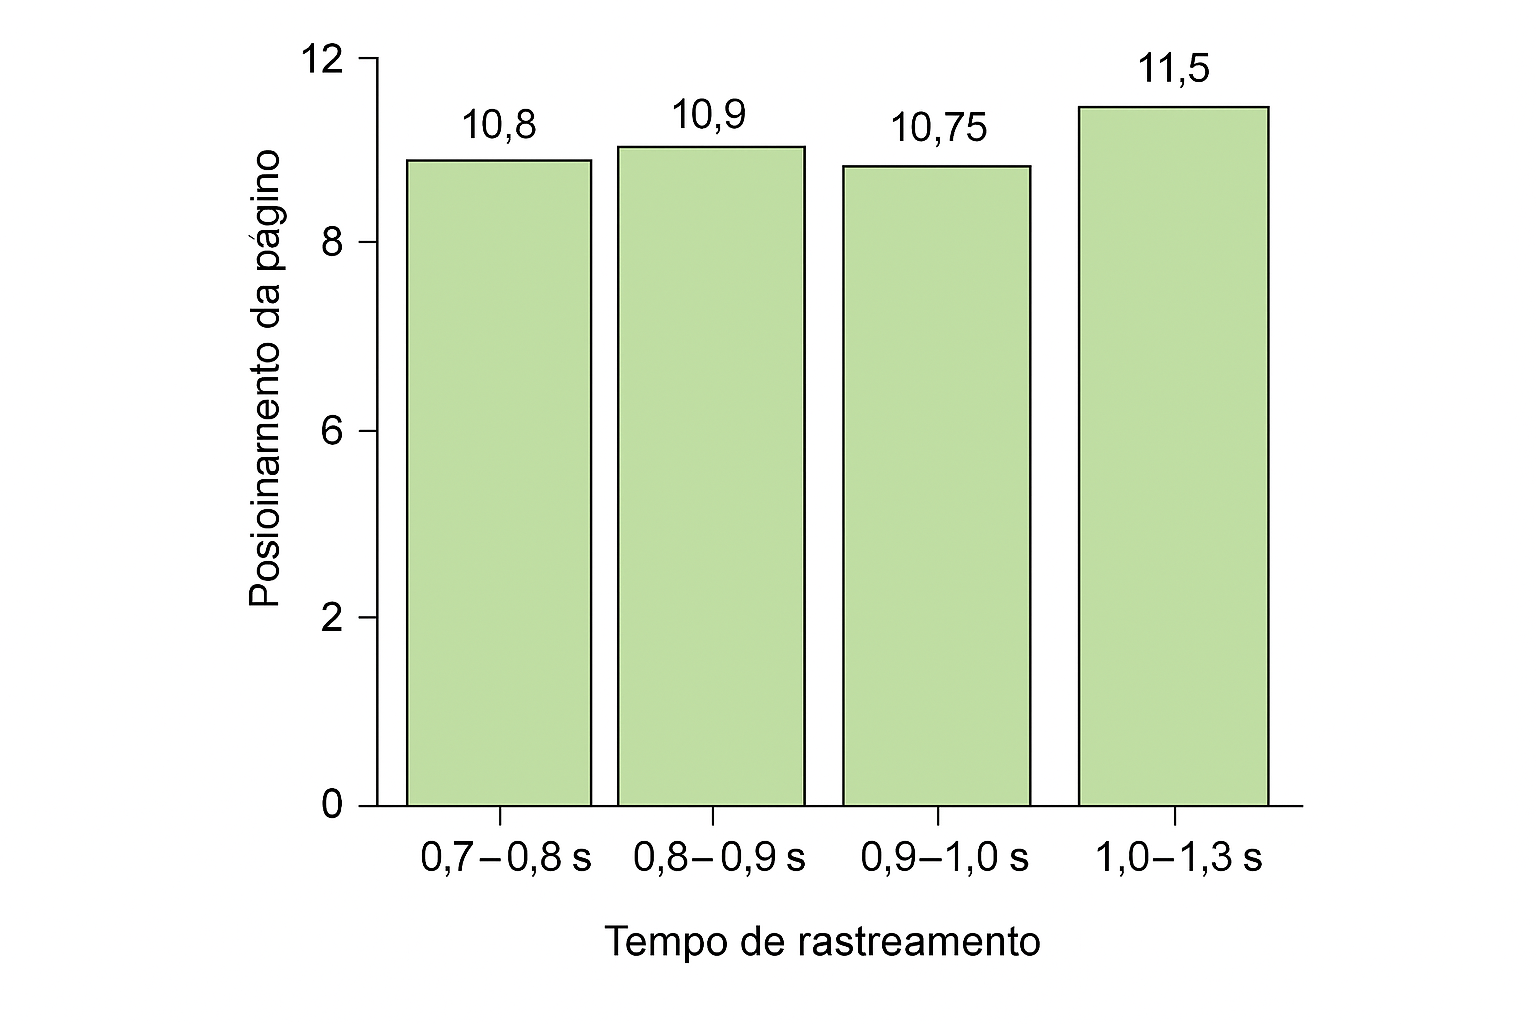
\includegraphics[width=0.6\textwidth]{media/rank_crawl_and_page_rank.png}
    \legend{Fonte: \cite{webPerformance}(adaptado)}
    \label{fig:rank_crawl_and_page_rank}
\end{figure}

A \autoref{fig:rank_crawl_and_page_rank} ilustra a relação entre o tempo de rastreamento e o posicionamento da página. O tempo de rastreamento refere-se ao tempo que os mecanismos de busca levam para acessar e indexar uma página. Quanto mais rápido o tempo de rastreamento, maior a probabilidade de a página ser indexada rapidamente e, consequentemente, melhor seu posicionamento nos resultados de busca. Isso destaca a importância de otimizar o desempenho do site para garantir uma boa classificação nos motores de busca.

\subsection{\english{Velocidade de carregamento}}
\label{sec:velocidade da página}

A velocidade de carregamento de uma página refere-se ao tempo necessário para que todo o seu conteúdo esteja visível e interativo no navegador, desde a solicitação inicial do usuário. Esse tempo pode ser influenciado por diversos fatores, como o tamanho dos arquivos, a complexidade do conteúdo, a qualidade da conexão com a internet e o desempenho do servidor \cite{shopify2024}.

Esse fator é determinante tanto para a \acrshort{ux} quanto para o \acrshort{seo}. Páginas que carregam rapidamente tendem a apresentar menores taxas de rejeição e melhores resultados em métricas de conversão. Além disso, o \acrshort{seo} utiliza a velocidade de carregamento como um dos critérios de ranqueamento nos mecanismos de busca \cite{conor2022}.

De acordo com \citeonline{google}, quanto mais rápido um site carregar, melhor tende a ser a experiência do usuário. Sites lentos comprometem a navegação e reduzem o tempo de permanência, afetando negativamente o engajamento.

A percepção de desempenho — muitas vezes chamada de \emph{velocidade percebida} — também é um fator crucial para a usabilidade e pode ser tão relevante quanto o tempo de carregamento real. Nesse sentido, a escolha entre \acrshort{ssr} e \acrshort{csr} influencia diretamente essa percepção. O \acrshort{ssr} geralmente proporciona carregamento inicial mais rápido, pois o conteúdo é renderizado no servidor e entregue ao navegador já pronto para exibição. Isso permite que os usuários visualizem o conteúdo principal imediatamente, mesmo que outros recursos ainda estejam sendo carregados \cite{atori2024}.

Por outro lado, no \acrshort{csr}, o navegador precisa baixar, interpretar e executar o JavaScript antes de renderizar qualquer conteúdo. Isso pode resultar em uma exibição inicial em branco ou em telas de carregamento, o que compromete a percepção de desempenho — especialmente em conexões lentas ou dispositivos com menor capacidade de processamento \cite{pixelfree2023}.


\subsection{Interatividade}
\label{subsec:interatividade}

A interatividade é um fator decisivo na experiência do usuário em aplicações web modernas, pois determina a forma como os usuários percebem a continuidade e a capacidade de resposta durante a navegação. Nas aplicações que utilizam \acrshort{csr}, o código JavaScript é executado diretamente no navegador, permitindo respostas imediatas a interações como cliques, preenchimento de formulários ou navegação entre páginas internas. Essa abordagem possibilita transições de página mais suaves e experiências semelhantes às de aplicativos nativos, sem a necessidade de recarregamentos completos \cite{pixelfree2023}.

Segundo \citeonline{atori2024}, a renderização no lado do cliente favorece experiências altamente dinâmicas, oferecendo um nível elevado de controle sobre os elementos da interface. Em contrapartida, o \acrshort{ssr}, embora proporcione carregamento inicial mais rápido e visibilidade imediata do conteúdo, apresenta limitações em termos de interatividade. Alterações na interface em aplicações \acrshort{ssr} geralmente demandam comunicações adicionais com o servidor, o que pode comprometer a continuidade da experiência do usuário \cite{atori2024, splunk2023}.

Para mitigar essas limitações, abordagens híbridas têm sido amplamente adotadas. Nelas, o conteúdo é inicialmente renderizado no servidor e, posteriormente, reativado no cliente com JavaScript, em uma estratégia conhecida como \emph{hydration} \cite{splunk2023}. Essa técnica busca aliar os benefícios de desempenho e \acrshort{seo} do \acrshort{ssr} com a interatividade aprimorada do \acrshort{csr}.


\subsection{Acessibilidade}
\label{subsec:acessibilidade}

A acessibilidade em aplicações web refere-se à capacidade de tornar conteúdos e funcionalidades utilizáveis por pessoas com deficiência, como visual, auditiva, motora ou cognitiva. É um princípio essencial para garantir a equidade no acesso à informação e à interação digital. De acordo com \cite{pixelfree2023access}, acessibilidade diz respeito a assegurar que todos, independentemente de suas habilidades, possam acessar e interagir com o conteúdo da web. Para pessoas com deficiência, isso pode significar o uso de leitores de tela, navegação por teclado ou a dependência de outras tecnologias assistivas.

As abordagens de renderização, como \acrshort{csr} e \acrshort{ssr}, impactam diretamente a acessibilidade, especialmente na compatibilidade com essas tecnologias. Em aplicações que utilizam \acrshort{csr}, o conteúdo geralmente é carregado de forma assíncrona após a execução do JavaScript, o que pode dificultar a leitura imediata por leitores de tela que dependem de uma estrutura HTML previamente carregada para interpretar a página corretamente \cite{pixelfree2023access}. Já no \acrshort{ssr}, o conteúdo é entregue completamente no carregamento inicial, facilitando a interpretação por essas ferramentas e proporcionando uma experiência mais estável para usuários com deficiência visual \cite{atori2024}.

Além disso, em contextos com atualizações dinâmicas de conteúdo — como ocorre em SPAs com \acrshort{csr} — é necessário adotar práticas específicas para garantir a acessibilidade, como gerenciamento de foco, uso de alertas ARIA e atualização de leitores de tela após mudanças no DOM. Essas medidas são fundamentais para que as mudanças de visualização sejam percebidas corretamente por tecnologias assistivas, uma vez que alterações no DOM nem sempre são reconhecidas automaticamente por leitores de tela. O envio de foco a elementos interativos ou o uso de regiões ARIA ao vivo são técnicas recomendadas para anunciar mudanças de estado ao usuário \cite{sutton2018}.

Assim, embora o \acrshort{ssr} ofereça uma base naturalmente mais acessível, ambas as abordagens podem ser igualmente inclusivas quando aplicadas com atenção às diretrizes e boas práticas de acessibilidade.


